\documentclass[border=5pt]{standalone}
\usepackage[T1]{fontenc}
\usepackage[utf8]{inputenc}
\usepackage{tikz}
\usepackage{amsmath}
\usepackage{FiraSans}
\newcommand{\tsf}[1]{\usefont{T1}{FiraSans-LF}{regular}{n}\fontsize{0.94em}{1em}\selectfont#1}
\usetikzlibrary{positioning, arrows.meta, calc}

\definecolor{tanfill}{RGB}{222, 200, 163}
\definecolor{grayfill}{RGB}{220, 220, 220}
\definecolor{tanborder}{RGB}{180, 160, 120}
\definecolor{grayborder}{RGB}{160, 160, 160}
\definecolor{bmidnight}{rgb}{0.0, 0.329, 0.576}

\begin{document}
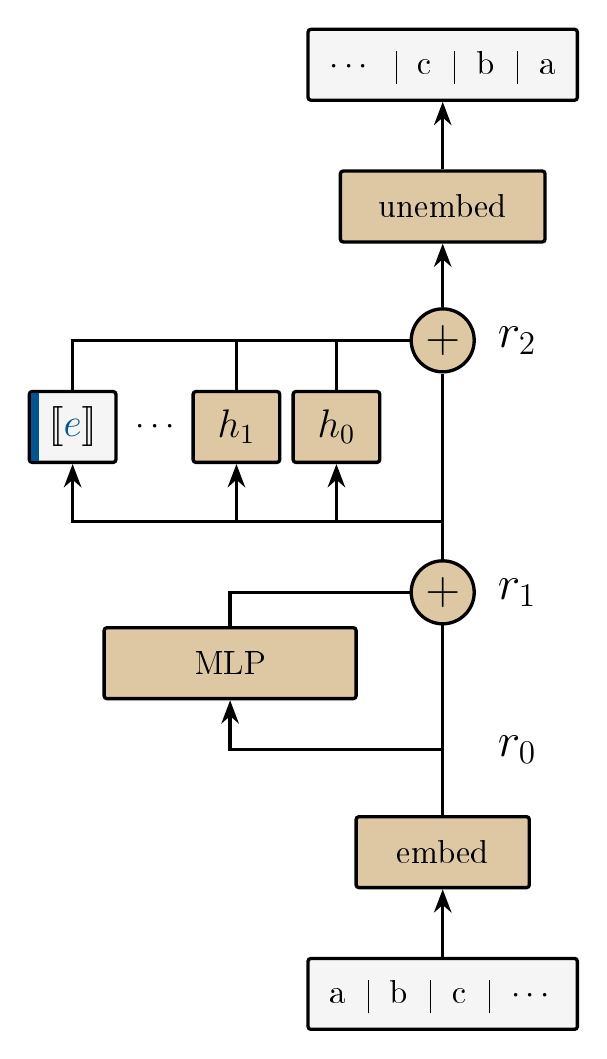
\begin{tikzpicture}[
    >=Stealth,
    every node/.style={line width=1.2pt},
    block/.style={
        draw=black,
        fill=#1fill,
        minimum width=2.2cm,
        minimum height=0.9cm,
        font=\Large,
        rounded corners=1pt,
    },
    head/.style={
        draw=black,
        fill=tanfill,
        minimum width=1.1cm,
        minimum height=0.9cm,
        font=\Large,
        rounded corners=1pt,
    },
    sumnode/.style={
        draw=black,
        fill=tanfill,
        circle,
        inner sep=0pt,
        minimum size=0.8cm,
        font=\LARGE,
    },
    stream/.style={->, very thick},
    dotstream/.style={->, very thick, densely dotted},
    branchout/.style={->, very thick},
    branchin/.style={->, very thick},
    plain/.style={very thick},
    plaindot/.style={very thick, densely dotted},
]

% -- Residual stream x-coordinate
\def\streamx{2.0} 

% -- Bottom: tokens
\node[draw=black, line width=1.2pt, fill=gray!8, minimum height=0.9cm, rounded corners=1pt, inner sep=0pt, text depth=1.5pt] (tokens) at (\streamx, 0.6) {%

    \begin{tabular}{c|c|c|c}
    \,\Large\tsf{a}\, & \,\Large\tsf{b}\, & \,\Large\tsf{c}\, & \,\Large\tsf{$\cdots$}\,
    \end{tabular}%
};

% -- Embed
\node[block=tan] (embed) at (\streamx, 2.4) {\tsf{embed}};

% -- Stream labels and nodes
\coordinate (streami) at (\streamx, 3.7);

% -- MLP
\node[block=tan, minimum width=3.2cm] (mlp) at (-0.7, 4.8) {\tsf{MLP}};

% -- Sum node after MLP
\node[sumnode] (sum1) at (\streamx, 5.7) {$+$};

% -- Attention heads
\node[head, fill=gray!8] (hn) at (-2.7, 7.8) {$[\![{\color{bmidnight}e}]\!]$};
\fill[bmidnight, rounded corners=0.0pt] ([xshift=1.2pt, yshift=1.1pt]hn.south west) rectangle ([xshift=1.4mm, yshift=-1.1pt]hn.north west);
\node[font=\Large] (hdots) at (-1.62, 7.8) {\tsf{$\cdots$}};
\node[head] (h0) at (-0.62, 7.8) {$h_1$};
\node[head] (h1) at (0.65, 7.8) {$h_0$};

% -- Sum node after attention
\node[sumnode] (sum2) at (\streamx, 8.9) {$+$};

% -- Unembed
\node[block=tan, minimum width=2.6cm] (unembed) at (\streamx, 10.6) {\tsf{unembed}};

% -- Logits
\node[draw=black, line width=1.2pt, fill=gray!8, minimum height=0.9cm, rounded corners=1pt, inner sep=0pt, text depth=1.5pt] (logits) at (\streamx, 12.4) {%
    \begin{tabular}{c|c|c|c}
    \,\Large\tsf{$\cdots$}\, & \,\Large\tsf{c}\, & \,\Large\tsf{b}\, & \,\Large\tsf{a}\,
    \end{tabular}%
};

% ===== Arrows =====

% tokens -> embed (arrow: into embed)
\draw[stream] (tokens) -- (embed);

% embed -> streami (no arrow)
\draw[plain] (embed) -- (streami);
\node[font=\LARGE, right=2pt] at ([xshift=2pt]sum1.east |- streami) {$r_0$};

% stream branches left to MLP (arrow: into MLP)
\draw[branchout] (streami) -| ([xshift=0pt]mlp.south);

% stream continues up to sum1 (no arrow)
\draw[plain] (streami) -- (sum1);

% MLP -> sum1 (no arrow)
\draw[plain] (mlp.north) |- (sum1.west);

% sum1 label
\node[font=\LARGE, right=2pt] at ([xshift=2pt]sum1.east) {$r_1$};

% stream branches left to attention heads (arrow: into heads)
\coordinate (attnbranch) at (\streamx, 6.6);
\draw[branchout] (attnbranch) -| (hn.south);
\draw[branchout] (attnbranch) -| (h0.south);
\draw[branchout] (attnbranch) -| (h1.south);

% stream continues up to sum2 (no arrow)
\draw[plain] (sum1) -- (sum2);

% attention heads -> sum2 (no arrow)
\draw[plain] (hn.north) |- (sum2.west);
\draw[plain] (h0.north) |- (sum2.west);
\draw[plain] (h1.north) |- (sum2.west);

% sum2 label
\node[font=\LARGE, right=2pt] at ([xshift=2.0pt]sum2.east) {$r_2$};

% sum2 to unembed (arrow into unembed)
\draw[stream] (sum2) -- (unembed);

% unembed -> logits (arrow: into logits)
\draw[stream] (unembed) -- (logits);

\end{tikzpicture}
\end{document}
